\section{Results}
\label{sec:results}
The results follow the ladder from cohort whitening to pool-basis whitening: first the accuracy of every rung, then the contrasts between adjacent rungs, and finally the diagnostics that explain why the oracle weights change nothing. The reused arms reproduce the values of the source studies exactly, because they are the same fits on the same bootstrap replicates.

\subsection{Accuracy along the ladder}
\label{sec:ladder-results}
The oracle-weighted within-patient arm lands exactly where the tuned patch-level arm does, and the pool's complement eigenbasis lands close to pool-basis whitening (Table~\ref{tab:ladder}). On TCGA-UT, Wo5 reaches 65.18 percent against 65.19 for Wt5, a gain of 0.44 points over cohort whitening (0.27 to 0.61). Po5 reaches 66.86 percent, a gain of 2.12 points (1.78 to 2.45) of the 2.66 points that separate cohort-basis from pool-basis whitening. Random directions with oracle weights gain 0.02 points ($-0.00$ to 0.05), as the random control with patch-level weights did. BRACS shows the same order with wider intervals: Wo5 gains 0.32 points ($-0.31$ to 0.94), Ro5 0.05 ($-0.02$ to 0.21), and Po5 2.33 (0.97 to 3.88) of a 3.01-point gap.

\begin{table}[htbp]
\centering
\footnotesize
\setlength{\tabcolsep}{4pt}
\renewcommand{\arraystretch}{1.15}
\begin{tabular}{@{}lrrrr@{}}
\toprule
 & \multicolumn{2}{c}{TCGA-UT} & \multicolumn{2}{c}{BRACS} \\
\cmidrule(lr){2-3}\cmidrule(lr){4-5}
Arm & Accuracy & Headroom & Accuracy & Headroom \\
\midrule
Real cohort (R5) & 62.48 [61.24, 63.65] & --- & 36.18 [33.46, 38.80] & --- \\
Cohort basis (RWc5) & 64.74 [63.52, 65.90] & 0 & 36.49 [33.87, 39.24] & 0 \\
Random, patch (Rt5) & 64.77 [63.54, 65.93] & --- & 36.56 [33.91, 39.27] & --- \\
Random, oracle (Ro5) & 64.76 [63.53, 65.93] & 0.007 [$-$0.001, 0.018] & 36.54 [33.89, 39.26] & 0.015 [$-$0.009, 0.077] \\
Within, patch (Wt5) & 65.19 [63.95, 66.34] & 0.169 [0.105, 0.231] & 36.94 [34.39, 39.48] & 0.149 [$-$0.140, 0.391] \\
Within, oracle (Wo5) & 65.18 [63.94, 66.32] & 0.166 [0.107, 0.228] & 36.81 [34.18, 39.46] & 0.106 [$-$0.126, 0.324] \\
Pool complement (Po5) & 66.86 [65.62, 67.99] & 0.796 [0.714, 0.880] & 38.82 [36.10, 41.27] & 0.773 [0.482, 1.031] \\
Pool basis (RW5) & 67.40 [66.14, 68.52] & 1 & 39.50 [36.82, 41.98] & 1 \\
Pool centres (C5) & 73.14 [71.62, 74.50] & --- & 44.63 [41.33, 48.05] & --- \\
\bottomrule
\end{tabular}
\caption{Oracle weights leave the within-patient arm where it was; only the pool's own complement directions close most of the whitening gap. Accuracy is test patient-macro balanced accuracy in percent at five patients per class; the headroom share is $(x-\mathrm{RWc5})/(\mathrm{RW5}-\mathrm{RWc5})$ and is 0 and 1 for the two whitening references by definition. Intervals are paired 95\% bootstrap intervals over test patients and draws. ``Cohort basis'' and ``Pool basis'' denote cohort and pool-basis whitening, ``Within'' and ``Random'' the within-patient and random complement directions, ``patch'' and ``oracle'' the added weights. R5, C5, RWc5, RW5, Wt5, and Rt5 are reused fits \citep{queisler2026centreError,queisler2026patientDirections,queisler2026bracsMechanism,queisler2026withinPatientSpan}.}
\label{tab:ladder}
\end{table}

\noindent Figure~\ref{fig:ladder} shows the headroom shares side by side. On both datasets the three arms whose added directions come from the cohort or from chance close less than a fifth of the gap, and the arm whose added directions come from the pool closes about four fifths. The step between the two groups is the change of direction, not the change of weight.

\begin{figure}[htbp]
\centering
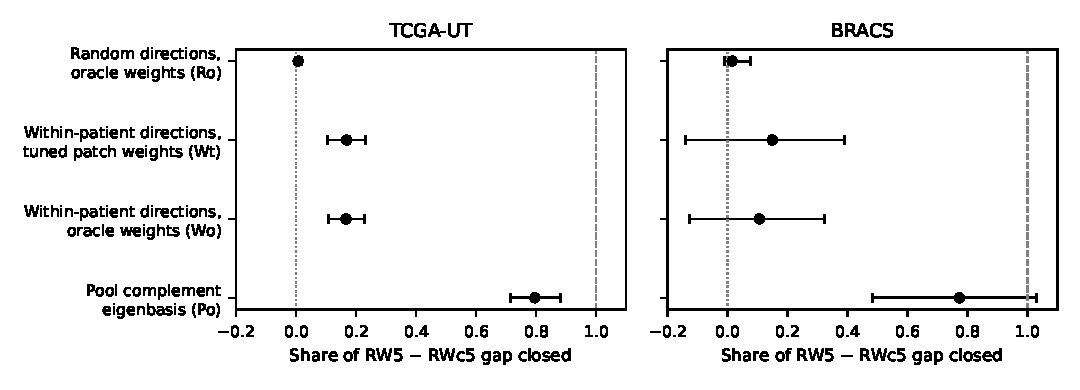
\includegraphics[width=\textwidth]{headroom_ladder.pdf}
\caption{Correcting the orientation of the added directions closes most of the whitening gap; correcting their weights closes no more of it than the tuned patch-level weights. Share of the gap between cohort whitening (dotted line, 0) and pool-basis whitening (dashed line, 1) closed by each arm at five patients per class, with paired 95\% bootstrap intervals.}
\label{fig:ladder}
\end{figure}

\subsection{Ladder contrasts}
\label{sec:contrast-results}
The primary contrast rejects the weight explanation on both datasets (Table~\ref{tab:contrasts}). On TCGA-UT, Wo5$-$Wt5 is $-0.01$ points, with an interval from $-0.11$ to 0.10 that excludes not only the one-point threshold but any gain larger than a tenth of a point. The difference is also stable across splits, at $-0.09$, 0.09, and $-0.02$ points. On BRACS the contrast is $-0.13$ points ($-0.73$ to 0.42); its upper bound lies well below the threshold, although the interval is five times wider.

\begin{table}[htbp]
\centering
\small
\renewcommand{\arraystretch}{1.15}
\begin{tabular}{@{}llrr@{}}
\toprule
Contrast & What it isolates & TCGA-UT & BRACS \\
\midrule
Wo5 $-$ Wt5 & Oracle against patch-level weights & \textbf{$-$0.01} [$-$0.11, 0.10] & \textbf{$-$0.13} [$-$0.73, 0.42] \\
Wo5 $-$ Ro5 & Within-patient against random directions & 0.42 [0.26, 0.59] & 0.27 [$-$0.35, 0.88] \\
Po5 $-$ Wo5 & Pool against within-patient orientation & 1.67 [1.37, 1.99] & 2.01 [0.74, 3.38] \\
RW5 $-$ Po5 & Cost of the block construction & 0.54 [0.31, 0.77] & 0.68 [$-$0.08, 1.62] \\
\addlinespace
Wo5 $-$ RWc5 & Oracle-weighted within-patient block & 0.44 [0.27, 0.61] & 0.32 [$-$0.31, 0.94] \\
Ro5 $-$ RWc5 & Oracle-weighted random block & 0.02 [$-$0.00, 0.05] & 0.05 [$-$0.02, 0.21] \\
Po5 $-$ RWc5 & Pool complement block & 2.12 [1.78, 2.45] & 2.33 [0.97, 3.88] \\
RW5 $-$ RWc5 & Whole gap & 2.66 [2.33, 2.97] & 3.01 [1.51, 4.68] \\
\bottomrule
\end{tabular}
\caption{The directions, not the weights, separate the within-patient block from the pool's complement block. Paired contrasts in percentage points at five patients per class with 95\% bootstrap intervals; bold entries are the primary contrast. The first four rows are the steps of the ladder RWc $\to$ Wt $\to$ Wo $\to$ Po $\to$ RW, apart from the step Wt$-$RWc reported by \citet{queisler2026withinPatientSpan}.}
\label{tab:contrasts}
\end{table}

\noindent The within-patient directions are better than random ones under the same oracle weights on TCGA-UT, by 0.42 points (0.26 to 0.59), which matches the specificity contrast Wt5$-$Rt5 of 0.42 points under patch-level weights \citep{queisler2026withinPatientSpan}. Correct weights therefore neither create nor remove the value of these directions. The largest step is the change of orientation: Po5 exceeds Wo5 by 1.67 points on TCGA-UT (1.37 to 1.99) and by 2.01 points on BRACS (0.74 to 3.38), and it does so in all three splits of both datasets. The last step, RW5$-$Po5, is 0.54 points on TCGA-UT (0.31 to 0.77), resolved but below the threshold, and 0.68 points on BRACS ($-0.08$ to 1.62), not resolved.

\subsection{Diagnostics}
\label{sec:diagnostics-results}
The diagnostics explain why oracle weights add nothing to the within-patient directions (Table~\ref{tab:diagnostics}). The patch-level variances $\omega_j$ rank the within-patient directions almost exactly as the pool's between-patient variance along them does: the Spearman correlation is 0.999 on TCGA-UT and 0.981 on BRACS, averaged over 30 fits. The oracle weights also imply an added trace of 0.296 times the cohort trace on TCGA-UT, which coincides with the best fixed value $s=0.3$ of the source study, and 0.412 on BRACS, where that study also peaked at $s=0.3$. Up to the exact shape of the profile, the tuned patch-level arm therefore already carried the oracle weights, both in ranking and in total size.

\begin{table}[htbp]
\centering
\small
\renewcommand{\arraystretch}{1.15}
\begin{tabular}{@{}lrrrrrr@{}}
\toprule
 & \multicolumn{3}{c}{TCGA-UT} & \multicolumn{3}{c}{BRACS} \\
\cmidrule(lr){2-4}\cmidrule(lr){5-7}
 & Wo5 & Ro5 & Po5 & Wo5 & Ro5 & Po5 \\
\midrule
Added directions & 2,438 & 2,438 & 2,440 & 1,085 & 1,085 & 227 \\
Added pool share & 0.302 & 0.301 & 0.302 & 0.401 & 0.181 & 0.423 \\
Oracle-implied added trace & 0.296 & 0.296 & 0.296 & 0.412 & 0.186 & 0.435 \\
Spearman$(\omega,\text{oracle})$ & 0.999 & --- & --- & 0.981 & --- & --- \\
\addlinespace
Selected factor 0.1 & 0 & 0 & 0 & 12 & 18 & 4 \\
Selected factor 1 & 5 & 23 & 0 & 7 & 6 & 2 \\
Selected factor 10 & 21 & 7 & 1 & 10 & 4 & 10 \\
Selected factor 100 & 4 & 0 & 29 & 1 & 2 & 14 \\
\bottomrule
\end{tabular}
\caption{On TCGA-UT all three added blocks carry the same pool variance in the same subspace; they differ only in how it is distributed over directions. Added directions and shares are means over 30 fits at five patients per class. The added pool share is the fraction of the pool's between-patient trace carried by the added block, and the oracle-implied added trace is that block's trace divided by the cohort trace. The selection rows count the scale factor, before rescaling, chosen in the 30 fits.}
\label{tab:diagnostics}
\end{table}

\noindent On TCGA-UT the three added blocks are indistinguishable by every span measure. Each spans the whole complement of the cohort basis and carries 0.30 of the pool's between-patient variance, which is all the pool variance outside the cohort basis \citep{queisler2026spectrumRegularization}. Yet Ro5 gains nothing, Wo5 gains 0.44 points, and Po5 gains 2.12. What distinguishes them is how the same trace is spread over directions, which is the property governed by the Schur--Horn majorization of Section~\ref{sec:model}: random directions spread it almost evenly, the within-patient directions concentrate it partly, and only the pool's eigenbasis concentrates it fully. On BRACS the within-patient complement covers 1,085 of the 2,532 complement directions but still carries 0.401 of the 0.423 pool share outside the cohort basis, whereas random directions of the same number carry 0.181. The pool's complement covariance there has rank 227 only, so Po5 concentrates the same variance on a fifth as many directions as Wo5.

The selected scale follows the concentration. On TCGA-UT, Ro5 keeps factor 1 in 23 of 30 fits, the choice of cohort whitening, and Wo5 selects factor 10 in 21 of 30 fits, as Wt5 did \citep{queisler2026withinPatientSpan}. Po5 selects the largest factor, 100, in 29 of 30 fits. Because the factors are anchored to the cohort block, this choice applies to both blocks a $\kappa$ one hundred times that of the factor cohort whitening usually selects, and validation still prefers it over every smaller factor. On BRACS, Po5 selects factor 100 in 14 and factor 10 in 10 of 30 fits, whereas Wo5 and Ro5 mostly select the smaller factors 0.1 and 1.

\section{Discussion}
\label{sec:discussion}
Of the four readings fixed in Section~\ref{sec:evaluation}, the results select the second on both datasets: Wo$\approx$Wt and Po$\gg$Wo. The explanation offered by \citet{queisler2026withinPatientSpan}, that the within-patient directions fail because they carry patch-level instead of patient-level weights, is rejected. Oracle weights change the accuracy by at most a tenth of a point on TCGA-UT, and the diagnostics show why: the patch-level variances already rank the within-patient directions as the pool does, and validation already chose the oracle trace. The first reading is excluded because the weights were not missing. The third is excluded because Po closes about four fifths of the gap. The fourth is excluded on TCGA-UT, where the within-patient directions beat random ones by the same 0.42 points under either weighting, and is unresolved on BRACS.

The bottleneck is the orientation of the added directions within the right subspace. On TCGA-UT, the within-patient complement, the random complement, and the pool's complement eigenbasis span the same space and carry the same pool variance, yet their gains are 0.44, 0.02, and 2.12 points. Whitening by Equation~\ref{eq:whiten} contracts each basis direction by its own weight and cannot represent variance that is shared between directions. The pool's between-patient variance outside the cohort basis is concentrated on comparatively few directions, and only a basis aligned with those directions contracts them strongly while leaving the rest of the complement, and the class signal in it, largely intact. In any other basis, the Schur--Horn theorem guarantees that the same variance appears more evenly spread, so whitening must either contract many directions moderately or few directions too weakly. The selected scale factors fit this picture: the concentrated Po block tolerates the strongest contraction on the grid, the partly concentrated Wo block a moderate one, and the nearly flat Ro block none beyond cohort whitening. The within-patient directions are informative, since they beat random directions, but their orientation reflects how patches vary within a patient, and that variation does not share the principal axes of patient-to-patient variation.

The result closes the line of cohort-only span remedies opened by \citet{queisler2026spectrumRegularization} and \citet{queisler2026withinPatientSpan}. The headroom outside the cohort basis is real and large, 2.12 of 2.66 points on TCGA-UT with the pool's complement eigenbasis, but it requires the principal axes of between-patient variation outside the cohort's span. Those axes are a property of the patient population. A cohort of five patients per class determines at most $C(G-1)$ of them, its patch residuals determine a different set of axes, and correct weights on the wrong axes recover nothing more. A remedy along these lines would have to estimate the population's between-patient axes from patients outside the labelled cohort, for example from unlabelled slides of further patients, since patient means require no labels.

The block construction itself costs little. Po keeps the cohort's eigenvalues on the cohort basis and drops the covariance between that basis and its complement, and still reaches 80 percent of pool-basis whitening on TCGA-UT. The remaining 0.54 points are resolved but below the practical threshold. Correcting the cohort eigenvalues alone is worth 0.08 points \citep{queisler2026spectrumRegularization}, so the remainder plausibly lies in the dropped cross-covariance or in the coarse scale grid; neither was isolated here.

\section{Limitations}
\label{sec:limitations}
All fitted arms read the between-patient covariance of the full training pool, so none of them is a remedy, and the study answers only where the bottleneck lies. It runs at five patients per class only; the source study found no gain at ten or twenty patients to explain, but the ladder at those counts was not measured.

The oracle weights are the diagonal of the pool covariance in the within-patient basis. This is the natural reading of ``patient-level weights'' for the whitening of Equation~\ref{eq:whiten}, which can only attach one weight to each basis direction, but it is not the only possible correction. A rotation within the within-patient complement that uses cohort-only information was not tried, and the conclusion that the orientation is the bottleneck applies to the within-patient eigenbasis as defined in Section~\ref{sec:model}. The Schur--Horn argument explains why a non-eigenbasis must spread the variance, but the eigenvalue profiles of the three blocks were not recorded, so the degree of concentration is inferred from the accuracy and the selected scale, not measured.

The scale grid limits Po. It selects the largest factor in 29 of 30 TCGA-UT fits, so a wider grid could raise Po5 and shrink the step RW5$-$Po5 further; the reported Po5 is a lower bound on the ceiling of the block construction, which strengthens rather than weakens the contrast Po5$-$Wo5. On BRACS, Po adds only 227 directions against 1,085 for Wo and Ro, so its contrast with them mixes orientation with a difference in the number of contracted directions, and all BRACS intervals are wide. The arms reuse the three evaluation splits of every earlier study in this series. The results are conditional on frozen Virchow2 features, multinomial logistic regression, 160 patches per class, and the two cohorts studied.
